\subsection{Complete input-stratified common-summary results}\label{sec:coverage}
Positive non-diagonal published demands are stratified by demand and directed free-flow shortest-path time using empirical tertiles, with ties kept in the lower bin. Within each of nine cells, lexicographically sorted OD indices at zero-based positions $\lfloor N/3\rfloor$ and $\lfloor2N/3\rfloor$ are retained. No attribution values enter selection. Endpoint differences identify total edge attribution, without identifying the same-state study/background response split. The two perturbation widths share every field of the selection protocol and differ only in the demand interval; their normalized errors are close for every query, so Table~\ref{tab:coveragefull} reports both in one table. Absolute minima, maxima, midpoints and half-ranges for both widths, and the per-position account sequences behind the segmentation of Proposition~\ref{prop:segmented}, accompany the result arrays in the code package.
\begin{table}[pos=htbp]\centering\footnotesize\caption{Complete geometric common summaries for the 18 input-stratified queries at both widths. Normalized error is Eq.~\eqref{eq:normerror} at $\pm10\%$ and $\pm20\%$; ranges are $[\phi_{\min},\phi_{\max}]$ at $\pm20\%$ in Sioux Falls cost units; P and M mean positive and mixed signs at $\pm20\%$.}\label{tab:coveragefull}\begin{tabular}{lrrrrl}\toprule OD & System & Range ($\pm20\%$) & Norm.\ err.\ ($\pm10\%$) & Norm.\ err.\ ($\pm20\%$) & Sign\\\midrule
(4,3) & 507.2 & [429.0, 535.0] & 9.9 & 9.9 & P\\
(12,3) & 337.2 & [330.7, 340.2] & 1.4 & 1.4 & P\\
(6,1) & 2360.6 & [658.3, 2290.4] & 35.6 & 35.6 & P\\
(15,6) & 9390.2 & [415.4, 4433.5] & 45.3 & 45.3 & P\\
(6,21) & 4577.8 & [-3.4, 2349.4] & 50.1 & 50.1 & M\\
(18,14) & 3422.3 & [150.8, 1929.7] & 46.1 & 46.1 & P\\
(8,4) & 25097.5 & [1270.7, 15741.3] & 46.0 & 46.0 & P\\
(19,8) & 16939.7 & [733.2, 7266.4] & 45.0 & 45.0 & P\\
(11,6) & 6165.9 & [1236.4, 6106.4] & 39.9 & 39.9 & P\\
(16,2) & 17763.1 & [896.3, 9628.6] & 45.3 & 45.3 & P\\
(8,21) & 7605.5 & [752.6, 4214.1] & 41.1 & 41.1 & P\\
(14,8) & 17445.3 & [890.3, 7527.1] & 44.1 & 44.1 & P\\
(11,15) & 47925.5 & [17628.9, 27737.8] & 18.2 & 18.2 & P\\
(17,9) & 24040.9 & [5482.3, 18519.3] & 35.2 & 35.2 & P\\
(10,12) & 55214.5 & [9822.4, 33248.6] & 35.2 & 35.2 & P\\
(13,10) & 54411.9 & [2918.8, 31345.2] & 45.3 & 45.3 & P\\
(1,10) & 33917.2 & [2182.9, 20856.4] & 44.8 & 44.8 & P\\
(10,1) & 34264.5 & [2182.7, 21039.5] & 44.8 & 44.8 & P\\
\bottomrule\end{tabular}\end{table}

\begin{figure}[pos=htbp]\centering
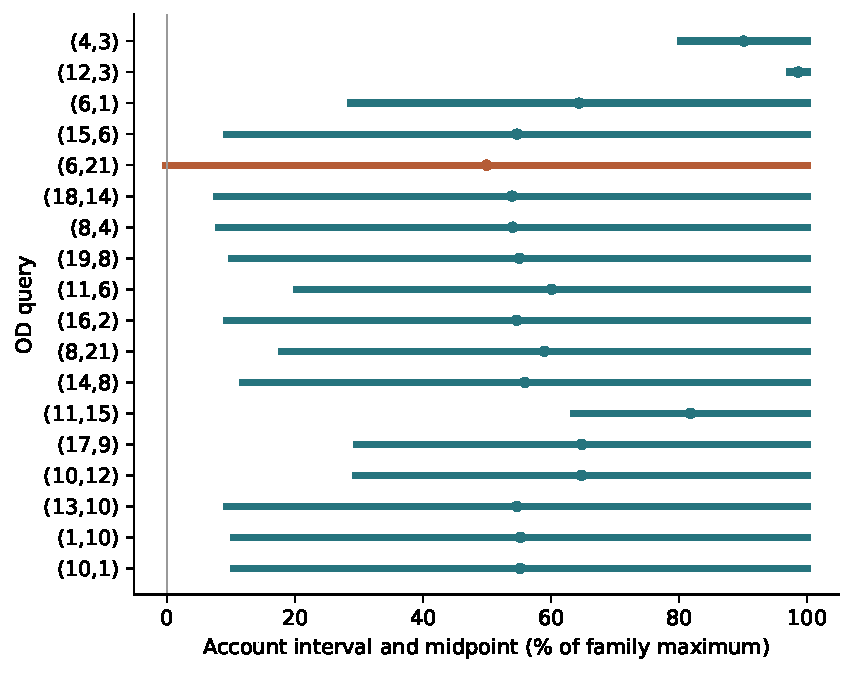
\includegraphics[width=0.88\linewidth]{../figures/fig_v106_coverage_intervals.pdf}
\caption{Geometric account intervals normalized by each query's largest
account magnitude, over all 18 input-stratified queries at $\pm20\%$
(the complete-interval companion of
Figure~\ref{fig:commonsummary}).}\label{fig:coverageintervals}
\end{figure}
